% gemmlir.tex -- LNCS full paper, built on samplepaper.tex (LLNCS v2.21).
% Compile: pdflatex gemmlir && pdflatex gemmlir
%
\documentclass[runningheads]{llncs}
%
\usepackage[T1]{fontenc}
\usepackage{graphicx}
\usepackage{amsmath}
\usepackage{amssymb}
%
\begin{document}
%
\title{gemmlir: End-to-End int8 Offload of PyTorch Models\\
to a Gemmini Systolic Array through MLIR}
%
\titlerunning{gemmlir: End-to-End int8 Offload through MLIR}
%
\author{Jaemin Kim\inst{1}\orcidID{0000-0000-0000-0000}}
%
\authorrunning{J. Kim}
%
\institute{Yonsei University, Seoul, Republic of Korea\\
\email{jaemin.kim@yonsei.ac.kr}}
%
\maketitle
%
\begin{abstract}
Systolic-array accelerators such as Gemmini are usually driven by hand-written C:
one call per layer, weights packed ahead of time. Step outside the shipped
workloads and there is no path at all. We present \emph{gemmlir}, an out-of-tree
MLIR dialect and pass pipeline that takes an unmodified PyTorch module through
torch-mlir, quantizes it to per-tensor int8, and emits a RISC-V object in which
every contraction is an accelerator call. The observation that organizes the
compiler is that a call is worth having only when a layer's whole \emph{tail} ---
bias, requantization, activation and pooling --- fits the shape the hardware's
output pipeline expresses; a layer that just misses is one to two orders of
magnitude slower than one that fits, so most of the work is rewrites that put
tails into that shape. Hardware and ABI constraints live in operation verifiers,
so a rewrite that cannot be expressed declines rather than approximates, and the
accelerator's numerics are reproduced exactly by a host reference. On a
Rocket+Gemmini U280 FPGA build, a regression set of 56 models compiles; fourteen
named architectures, including twelve from torchvision and the four MLPerf Tiny
benchmarks, put every contraction on the accelerator, run 19$\times$ to
2912$\times$ faster than the identical object with the accelerator removed, and
are byte-identical to it over forty runs each. Over twelve real models the accelerator is
12\% of 8.06\,s, and the calls that dominate are bandwidth-starved rather than
compute-bound.

\keywords{MLIR \and Deep learning compilers \and Quantization \and Systolic
arrays \and RISC-V \and Hardware accelerators.}
\end{abstract}
%
\section{Introduction}

A deep-learning accelerator is only as reachable as its software. Gemmini
\cite{gemmini} is the most widely used open systolic-array generator for RISC-V:
it produces a Rocket \cite{rocket} co-processor with a 16$\times$16 INT8 array, a
scratchpad, an accumulator and a scale-and-saturate output pipeline, and ships a
runtime header with tiled entry points for matmul, convolution and residual
addition. What it does not ship is a compiler. Its distributed workloads are
hand-written C --- one call per layer, weights packed offline, shapes baked in ---
and grouped convolutions, channel shuffles, dilation, transposed convolutions and
attention do not appear in them at all. A user with a PyTorch model and a Gemmini
bitstream has no path between the two.

The obvious path is MLIR \cite{mlir}: export through torch-mlir \cite{torchmlir}
to \texttt{linalg}, where a \texttt{linalg.matmul} is, on its face, what the
runtime's tiled matmul computes. In practice almost nothing about a real model
arrives in that form --- NCHW convolutions where the runtime reads NHWC, batch
normalization as a per-channel affine the single output scale cannot express, a
pool in float where the hardware wants one on bytes, a residual add inside the
same region as a requantization the hardware would do for free.

These mismatches are not gradual, and that is the central empirical fact here.
Gemmini's value is concentrated not in the multiply but in the \emph{mvout
pipeline}: leaving the accumulator, a value has a per-column bias added, is
multiplied by one scale, passes an activation, is saturated to int8 and may be
max-pooled --- all in hardware, all free. A layer whose tail is exactly that chain
becomes one call; a layer whose tail is that chain plus one operation the pipeline
does not have becomes a scalar loop on a 62.5\,MHz in-order core, with an address
computation per multiply-accumulate. On one two-convolution network, folding both
convolutions gave 2.49\,ms; folding only the first gave 25.8\,ms, worse than
folding neither and going through an im2col matmul (5.44\,ms). Offload is
all-or-nothing per layer, so the compiler's job is less instruction selection than
\emph{reshaping a quantized model's tails} until they fit.

Throughout, the baseline and the correctness oracle are one thing: the identical
compiled object linked twice, once against the accelerator runtime and once
against a host implementation of the same surface, required to agree byte for
byte.

\section{Background}

Gemmini \cite{gemmini} generates a RoCC co-processor for a Rocket core
\cite{rocket}. Our configuration on a Xilinx U280 has a 16$\times$16 INT8 array
(256\,MAC/cycle), four scratchpad banks of 4096 rows and two accumulator banks of
512, and runs Linux at 62.5\,MHz. Software reaches it through \texttt{gemmini.h},
whose tiled entry points we treat as the ABI; tiling is the runtime's. Three
properties shape everything downstream. The
\textbf{mvout pipeline is free}, as above. It is \textbf{one scale and one bias
shape}: a single scale per call, a single \texttt{D} pointer, and a $1{\times}N$
bias broadcast \emph{down} the rows, i.e.\ per column --- no per-row form, no
per-channel scale. And the \textbf{convolution entry points always requantize}:
\texttt{tiled\_conv\_auto} writes int8 and has no form that hands back the i32
accumulator, so a convolution whose result the model needs in float has nowhere to
go, while \texttt{tiled\_matmul\_auto} \emph{does} have such a form --- which is
why a 1$\times$1 convolution rewritten as a matmul offloads where the same layer
as a convolution cannot. Weight-stationary is also the only correct int8
dataflow here: output-stationary accumulates in 20-bit processing-element
registers, and an int8 product reaches $2^{14}$, so any $K$ past about 32 is
wrong.

MLIR \cite{mlir} provides the dialect infrastructure, \texttt{linalg}
\cite{linalgcodegen} structured operations with explicit indexing maps, and
torch-mlir \cite{torchmlir} an export path from PyTorch \cite{pytorch}. Three gaps recur. \emph{Layout}: PyTorch lowers to \texttt{conv\_2d\_nchw\_fchw}
while the runtime reads (KH, KW, C, F), linalg's \texttt{nhwc\_hwcf}.
\emph{Spelling, not semantics}: a batch of one is written as a constant
\texttt{0} in an indexing map rather than a loop dimension, so
\texttt{isIdentity()} answers ``no'' about a map that computes the identity, and
any check phrased as a question about a map's spelling is wrong. And one concept has several spellings: a global average pool
arrives as \texttt{nn.AdaptiveAvgPool2d}, \texttt{F.adaptive\_avg\_pool2d} or
\texttt{x.mean(dim=(2,3))}, reaching linalg as three different operations.

We use symmetric per-tensor quantization \cite{jacob,krishnamoorthi}: $q =
\mathrm{round}(x/s)$ with $s = \max|x|/127$, saturated to $[-128,127]$, so a
contraction accumulates in i32 at scale $s_A s_B$ and the tail rescales to the
consumer's scale --- exactly what the mvout does. That, rather than accuracy, is
why the scheme is per-tensor: the hardware applies one scale per call, so a per-channel
scale cannot fold into it.

\begin{figure}[t]
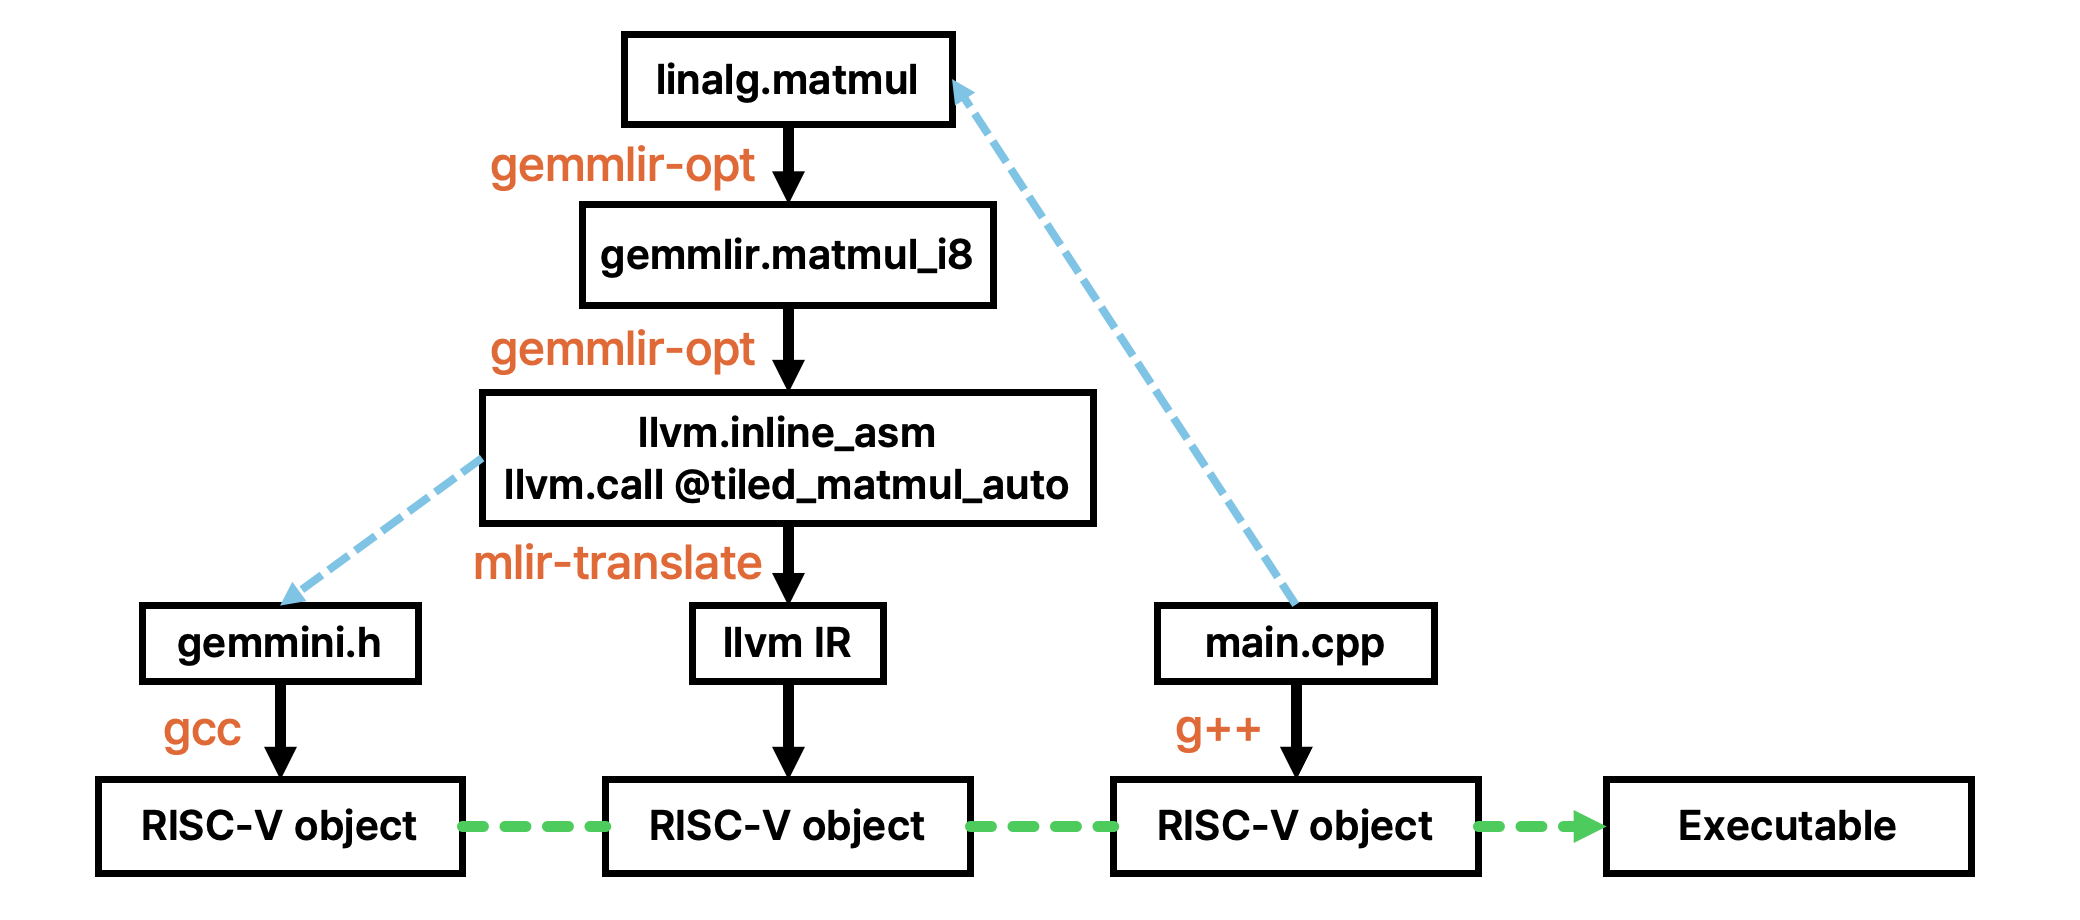
\includegraphics[width=\textwidth]{gemmlir-pipeline.png}
\caption{The toolchain on its simplest input: a \texttt{linalg.matmul} on memrefs
becomes a \texttt{gemmlir.matmul\_i8}, then an \texttt{llvm.call} to the runtime
preceded by an inline-assembly \texttt{gemmini\_flush}, then LLVM IR and a RISC-V
object linked against a compiled \texttt{gemmini.h} and a driver. The quantized
path inserts some forty rewrites above the first arrow.}
\label{fig:toolchain}
\end{figure}

\section{The gemmlir Dialect}
\label{sec:dialect}

The dialect is thin: one operation per runtime entry point (Table~\ref{tab:ops}),
plus a \texttt{memset} helper. The driver chains \texttt{gemmlir-opt},
\texttt{mlir-translate} and \texttt{llc} (Fig.~\ref{fig:toolchain}) in four
phases: a \emph{frontend} on tensors that normalizes layout and raises pools to
contractions --- all before calibration, because a pass that manufactures a
contraction manufactures something whose activation range has to be measured ---
then \emph{quantization} and bufferization, then \emph{offload} on memrefs, then
\emph{host code generation}. A matched layer looks like this --- a 7$\times$7 stride-2
convolution with padding 3, a per-channel i32 bias, a requantization, a ReLU and a
padded 3$\times$3 stride-2 max pool, which is the entry layer of every ImageNet
vision model, as one call:

\begin{footnotesize}
\begin{verbatim}
gemmlir.conv2d_i8(%in, %w, %out) bias(%d : memref<16xi32>)
    {stride = 2, padding = 3, act = #gemmlir.act<relu>,
     scale = 2.9411e-03 : f32, pool_size = 3, pool_stride = 2,
     pool_padding = 1}
  : (memref<1x64x64x3xi8>, memref<7x7x3x16xi8>, memref<1x16x16x16xi8>)
\end{verbatim}
\end{footnotesize}

\begin{table}[t]
\caption{The dialect's operations and the runtime calls they lower to. Each also
carries a \texttt{dataflow} attribute passed through as
\texttt{tiled\_matmul\_type}.}\label{tab:ops}
\footnotesize
\begin{tabular}{|l|l|}
\hline
operation & runtime call \\
\hline
\texttt{gemmlir.matmul\_i8} & \texttt{tiled\_matmul\_auto}, \texttt{full\_C} --- i32 accumulators out \\
\texttt{gemmlir.matmul\_i8\_scale} & \texttt{tiled\_matmul\_auto} --- scaled, saturated to i8, \texttt{act} applied \\
\texttt{gemmlir.resadd\_i8} & \texttt{tiled\_resadd\_auto} \\
\texttt{gemmlir.conv2d\_i8} & \texttt{tiled\_conv\_(stride\_)auto} --- bias, activation, pooling fused \\
\texttt{gemmlir.depthwise\_conv2d\_i8} & \texttt{tiled\_conv\_dw\_auto} \\
\texttt{gemmlir.norm\_i8} & \texttt{tiled\_norm\_auto} --- layernorm or I-BERT softmax \\
\hline
\end{tabular}
\end{table}

\paragraph{Verifiers as the hardware contract.} The runtime's parameters are
single integers, so only square kernels, strides, dilations and paddings are
expressible; the pooled extent is derived and a mismatch rejected; the depthwise
filter is read as (C, KH, KW), not linalg's (KH, KW, C); a reduction activation is
refused on a convolution, whose accumulator holds a window of pixels rather than a
row. Each is a verifier error rather than a matcher condition, so a run-time check
in the ABI becomes a compile-time one --- \texttt{tiled\_conv\_auto} exits on
\texttt{kernel\_dim <= padding} against the \emph{undilated} kernel, so a 3-tap
filter at dilation rate 4 is refused, its border stays materialized, and the layer
still offloads. A restriction discovered on hardware belongs there too: the runtime
addresses an NHWC buffer with one stride between two pixels, so a 16$\times$16
window inside an 18$\times$18 buffer has a wider row than it can express and the
accelerator writes the wrong rows with nothing reporting it --- which shipped
undetected in one model at 0.0106 relative $L_2$ where 0.0030 was available, inside
the range the others live in, and \emph{faster} than the correct version, because
writing 16 rows where 18 were meant is less work.

\paragraph{Numerics.} Two details make a host reference possible, and that
reference is what every correctness claim below rests on. The mvout rounds half to
\emph{even}, so a requantization that truncates is a different function and the
matcher requires an explicit \texttt{math.roundeven} --- for one
$32{\times}64 \times 64{\times}48$ matmul the two roundings differed in 790 of
1536 elements. And the compiler saturates as the mvout does, emitting
$\mathrm{trunci}(\mathrm{clamp}(\mathrm{fptosi}(\mathrm{roundeven}(x/s)),
-128,127))$ in i32 before narrowing. Lowering a \texttt{quant.qcast} does neither:
\texttt{arith.fptosi} is undefined outside the destination's range and on RISC-V
wraps, so an activation a little past $+127$ comes back as a large negative number
the moment an input exceeds what the calibration saw. Driving one model's input from 1$\times$ to 6$\times$ its
calibrated range, saturating degrades monotonically (0.0054 to 0.5896 relative
$L_2$) while wrapping jumps around (0.0054, 0.4341, 0.8785, 0.5744, \ldots) because
each wrap flips a sign. In range the two are bit-identical, and saturating costs
1.2\%.

\section{Quantization}
\label{sec:quant}

\paragraph{Scales.} A constant operand is measured at compile time, looking
through pure copies, since a frontend hands weights over behind a transposing
\texttt{linalg.generic}. An activation is annotated by a calibration script that
hooks the model's layers, records $\max|x|$ over representative inputs and writes
the attribute onto each contraction; matmuls are matched to layers by position and
checked against the shapes, and a mismatch raises rather than annotating, because
a scale on the wrong layer is worse than no scale --- a refusal that caught three
frontend gaps that would otherwise have produced a model that ran and was wrong.
The accumulator's scale is the product of the two, and this matters more than it
looks (Table~\ref{tab:scales}): the two matmuls of that MLP saw activations
reaching 3.74 and 2.11, so no single scale serves both. Two cases needed the calibration to
look elsewhere than a module's input. A transformer's $QK^{\!\top}$ and
$\mathrm{probs}\cdot V$ are the \texttt{@} operator on tensors rather than
modules, and both operands are activations where a convolution's right operand is
a constant: using the left operand's scale for the right gives 0.8352 relative
$L_2$ against 0.0115 once both are measured, since probabilities live in
$[0,0.13]$ and the values they weigh reach 2.8. A constant operand is also quantized \emph{at compile time}: the pass walks back
to the \texttt{arith.constant} through generics that only yield their input,
composing the permutation off the \emph{output} map, since that is the side a
frontend permutes to express a transpose. On a two-layer CNN that removed 4928 of
29520 elements and took the board from 18.82 to 15.39\,ms with the output
bit-identical. That walk is the most-repeated source of error in the project ---
four times a model was silently quantized at the wrong scale because it stopped
one operation short, costing up to 0.0126$\to$0.1295 relative $L_2$ --- so when a
pass falls back for want of a constant, the fallback must be loud. Ours warns, and
across 56 models exactly two operations take it.

\begin{table}[t]
\caption{Relative $L_2$ of a quantized MLP on the board against PyTorch's f32
output, as the scales become more specific. Simulating the same arithmetic in
PyTorch predicts the last two rows exactly, so nothing else in the pipeline loses
precision.}\label{tab:scales}
\centering
\footnotesize
\begin{tabular}{|l|c|}
\hline
scales & relative $L_2$ \\
\hline
one fixed 0.02 everywhere & 0.49 \\
weights measured, one activation scale for both layers & 0.20 \\
weights measured, per-operation activation scales & 0.036 \\
\ldots{}and rounding instead of truncating & \textbf{0.012} \\
\hline
\end{tabular}
\end{table}

\paragraph{The bias, into the accumulator.} A frontend writes a tail as
$\mathit{acc}\cdot s + b$ in float; the accelerator adds \texttt{D} to the i32
accumulator \emph{before} scaling, and since
$\mathit{acc}\,s + b = (\mathit{acc} + b/s)\,s$, a constant bias becomes
$\mathrm{round}(b/s)$ at compile time --- the standard int8 bias quantization,
whose error is half a step of $s$, the accumulator's own resolution. It fires only
where the bias could reach \texttt{D} and the result is requantized; on a network's
last layer the bias stays in float, which is strictly more accurate.

\paragraph{Sharing a quantization at a branch.} A residual block's input feeds both
the first convolution and the shortcut; the shortcut wants it in float, so the
producing layer's tail never ends in a requantization and does not fold --- 1 of 3
convolutions offloaded, 66.99\,ms. Quantizing the branch once and handing the other
consumers the dequantization of that value is what a quantized residual network
does anyway, and is the precondition for reaching \texttt{resadd\_i8}. Three things had to hold at once: the
dequantization must be written out as \texttt{sitofp} and a multiply rather than a
\texttt{quant.dcast}, since the quant dialect folds
$\mathrm{dcast}(\mathrm{qcast}(x))$ back to $x$ and the greedy driver then never
terminates with no diagnostic; the quantization must land in the convolution's
layout, since the matcher requires an identity write map while a frontend's tail is
NCHW; and fusion must not widen an i8 activation back to float, which would put the
widening inside the producer. The pass fires
either because the value comes off a quantized contraction, where the prize is that
the layer offloads at all, or because some consumer is quantizing the value anyway.
What makes the second case safe is that \textbf{the branches already agree on the
scale}: an LSTM's input is sixteen timesteps sliced from one tensor with scales
from 0.0128 to 0.0248, and hoisting one over all sixteen makes the widest timestep
saturate at the narrowest one's range, which was the whole of a
0.0066\,$\to$\,0.0284 regression. Three guards were tried and measured first, all of which left the LSTM at
0.0284; the right one was found by diffing the pass output under each candidate
rather than guessing a fourth, which showed the LSTM differing at one site of
160. On the board the pass is worth
550.76\,$\to$\,400.46\,ms on EfficientNet-B0, 273.28\,$\to$\,150.66 on
RegNetY-400MF and 65.42\,$\to$\,63.05 on ShuffleNetV2.

\paragraph{A layer that keeps its own requantization, and 256 answers.} Some
activations are not in the mvout's vocabulary: SiLU, hard-swish, GELU. A dense
convolution below one can fall back to an im2col matmul, which leaves an i32
accumulator for the float tail; a \emph{depthwise} one cannot, because
\texttt{tiled\_conv\_dw\_auto} writes i8 like the rest.
\texttt{--quantize-unfoldable-tails} cuts the tail into the part the call can do
and the part the core does afterwards, at the layer's \emph{own} output range,
which the calibration measures separately because the next layer's input range is
on the far side of the activation. The cost was simulated in PyTorch first:
0.00016 relative $L_2$ against a model whose own quantization error is 0.0186. The test for what blocks a tail
ended up narrower than ``which operations can the pipeline absorb'': what the call
cannot do is read its accumulator on \emph{two} paths at once, because the mvout
writes each output element from one accumulator, once --- and SiLU, hard-swish and
layer norm are all that shape. The cut has a consequence worth more than the offload it was written
for: the activation now reads a byte, and an elementwise chain below an i8 has 256
answers, so \texttt{--table-for-i8-elementwise} evaluates it at compile time into a
256-entry constant. The anchor is a value \emph{inside} the region, not the
operation's input, since fusion has already put the quantization, the
dequantization and the activation in one region and the byte never reaches memory.
Where a region computes from several i8 slices at once --- an LSTM gate is
$\sigma(f)c + \sigma(i)\tanh(g)$ --- the pass takes the largest value anywhere
in it that is a function of one byte, rather than asking about the value it
yields. EfficientNet 1913.8\,$\to$\,1115.7\,ms with relative $L_2$ unchanged; the
LSTM 37.55\,$\to$\,17.60\,ms at 0.0038\,$\to$\,0.0066; a ViT 955\,$\to$\,469\,ms
with no \texttt{erff} left. Models whose activations are ReLU grow no tables.

\section{Getting Whole Layers onto the Accelerator}
\label{sec:folding}

Every rewrite here puts a layer's tail into the shape the mvout expresses, or
removes something standing between two layers that would otherwise meet.

\paragraph{Layout.} \texttt{--conv-nchw-to-nhwc} rewrites NCHW convolutions,
depthwise convolutions and poolings into NHWC with explicit transposes, composes
those that meet, and pushes a transpose past the elementwise operations between two
layers; constant filters are permuted at compile time. The effect is
13.4\,$\to$\,5.4\,ms, but on its own the pass was a 25\% \emph{loss}, and the
reason is more useful than the number. MLIR's im2col rewrite contracts
$X(P \times CK_hK_w)\cdot W(CK_hK_w \times F)$ in NHWC, with channels in the
columns, and that one difference is what lets the rest of a quantized layer reach
the accelerator, because \texttt{repeating\_bias} is a row repeated \emph{down} the
rows --- per column. From NCHW the contraction comes out $W(F \times CK_hK_w)\cdot X(CK_hK_w \times
P)$, the bias is per row, there is no per-row \texttt{D}, and the whole tail
stays in software. The loss came from how the pack is written: MLIR collapses
the patch offset into $K$ and the position into $P$, so taking either apart
costs a floordiv and a mod per level, and which loop they land on decides how
often they run --- for NCHW the position, whose divisors are powers of two, and
for NHWC $K$, whose divisors are the kernel's 9 and 3. Writing the NHWC pack as a
nested loop $(n, o_h, o_w, k_h, k_w, c)$, where the indices \emph{are} the
offsets, removes the arithmetic, and a \texttt{collapse\_shape} afterwards is a
view: on one 6912-element pack, 3.79\,ms for MLIR's NCHW form and 9.21 for its
NHWC one, against \textbf{1.77}\,ms written out. Index arithmetic, not layout and
not locality.

\paragraph{Skipping im2col, and when not to.} Once the model is NHWC the detour can be dropped: the accelerator does not mind
either way (0.055\,ms direct against 0.064\,ms packed), and the direct call makes
the pack disappear --- one CNN dropped from 5.44 to 2.49\,ms. im2col is kept for
what the convolution provably cannot express: a result that reaches the return
still wide, a shape the hardware computes wrongly, or a non-square kernel (packing
a 1$\times$3 and a 3$\times$1 took one model from 27.95 to 4.64\,ms). The walk deciding this has been fooled four times, and each fix is a rule: an i8
below the convolution is not proof that something will fold into it
(EfficientNet's sat below a \emph{SiLU}, and 33 convolutions were declined for a
fold that was never going to happen); a requantization larger than anything the
convolution wrote cannot be the convolution's (a U-Net decoder,
25.5\,$\to$\,5.45\,ms); a reduction is not something the mvout does, even though
a layer norm's mean has a single \texttt{addf} for a body; and a value read
twice is not reached by a walk that stops at the first branch. Being wrong in
this direction costs a packed convolution that need not have been, never a wrong
answer.

\paragraph{Batch normalization.} In evaluation mode a batch norm \cite{batchnorm}
is a per-output-channel affine that nothing downstream can take. On one residual
block that is 117.5\,ms against 1.04. All of it is constant, so it goes into the
weights: scaling output channel $f$ of the filter by $a[f]$ scales that channel's
whole result, and the additive part joins what the convolution was already
accumulating onto. The pass does not pattern-match the formula: each value in the body is
classified as constant or as $a\cdot\mathit{in}+b$ and propagated forward,
refusing anything outside a small vocabulary, which covers a batch norm however
a frontend spells it. Folded, the
block goes from 1 call and 25366 scalar elements to 6 calls and 778, and the
accuracy is fractionally \emph{better} (0.0031\,$\to$\,0.0030), because the folded
form rounds twice where the original rounded three times.

\paragraph{Residual adds.} After branch sharing, the convolution still not folding
is the one whose tail \emph{is} the residual add --- one \texttt{linalg.generic}
reading a shortcut, an accumulator and a bias, which no single Gemmini call
expresses. \texttt{--split-residual-add} separates the convolution's own
requantization, which folds into the call, from the scaled add of two i8 tensors,
which is what \texttt{resadd\_i8} is. The intermediate is quantized at the block output's scale,
making the add exact and leaving one approximation: the convolution's result is
rounded to i8 where the fused form kept i32. That is a real numerical change
(0.0070 to 0.0097) and the reason it is a pass of its own. On one residual block
the four rewrites of this section compose: 2 offloaded calls and 15606 scalar
elements at 66.99\,ms, then 3 and 10538 at 43.17 once the branch is quantized in
the convolution's layout, then 4 and 3850 at 3.73 with the residual split out, then
5 and 1802 at \textbf{1.78} once the scaled add is matched to \texttt{resadd\_i8}
--- against 306.1\,ms for the same object with the runtime on the host.

\paragraph{Pooling and padding.} A frontend pools in float and requantizes afterwards, so the convolution's tail
has no i8 result to fold into. \texttt{max} commutes with any non-decreasing
function, so the requantization goes first and the pool runs on i8; only a body of
provably non-decreasing operations is moved, and a truncation counts only once a
clamp has made it safe. An average pool is a contraction, not a pool: in NHWC the
image already reads as $(HW,C)$, so a global mean is
$\mathbf{1}(1,HW)\cdot\mathrm{image}(HW,C)$ with the constant folded to i8 and the
divide absorbed into the call's requantization scale. Gemmini's own global average pool is the wrong tool, since it writes the mean at
the \emph{input's} scale and a mean over 256 pixels has a range that much
smaller. A padded max pool folds only with an argument: PyTorch pads with
$-\infty$ and Gemmini's out-of-bounds branch reads \emph{zero}, and the two agree
exactly when the pooled values cannot be negative, which the ReLU the convolution
already carries guarantees. A convolution's
padding needs no buffer at all, since the call applies it as it reads the image.
Over three such rewrites one model's entry layer went 89.8\,$\to$\,2.20\,ms.
Three further rewrites follow the same pattern: a requantization distributed over
a concatenation's pieces so each branch's tail folds, with the branch written into
a \texttt{memref.subview} of the join rather than copied (4.96\,$\to$\,0.95\,ms
on one block, GoogLeNet 1603.8\,$\to$\,1191.7); a grouped convolution split into
$G$ convolutions sliced in NHWC after one transpose in and one out, rather than
$G$ pairs of transposes; and a channel shuffle folded into the constant filter
(55.32\,$\to$\,2.31\,ms) --- with the \emph{inverse} permutation, which is a
different list unless the group sizes are equal, so getting it backwards is a
wrong answer rather than a rearranged one.

\section{Host-Side Code Generation}
\label{sec:host}

After offload what is left is the model's float/int8 boundary plus whatever did not
fold, and on this core that is most of the remaining time.
Each of the twenty-odd passes of this phase was measured on its own in a board
session where both objects were built, staged and alternated: the reciprocal
rewrite 12.7\% over 26 models, the two copy rewrites 9.3\% and 6.7\% over the
models that have copies, elementwise unrolling and \texttt{fma} about 4\% each,
and the relayout fold 27\% on the one model it applies to. The recurring lesson is
that on an in-order single-issue core what an element costs is its
\emph{dependency chain}, not its instruction count.

\paragraph{One static arena.} Bufferization allocates every intermediate; MobileNetV2's come to 4.45\,MB across
137 buffers, and with \texttt{mlockall(MCL\_FUTURE)} the kernel populates a mapping
at \texttt{mmap} time, so every inference paid for 4.45\,MB of fresh pages --- with
the accelerator calls nulled out an inference still took 55.67\,ms of its 124.11
with only 3082 scalar elements to compute, which at 80\,MB/s is what a 62.5\,MHz
core zeroing and locking pages looks like.
\texttt{--plan-static-buffers} makes every temporary a view into one uninitialized
\texttt{memref.global}, so the function allocates nothing and the addresses are
fixed by construction, which the hardware separately requires
(Section~\ref{sec:cache}). MobileNetV2 went 124.11\,$\to$\,66.52\,ms and every
other model gained 1--11\%; the cost is that the compiled function is \textbf{not
re-entrant}. Sharing the arena between buffers whose lives do not overlap would
save a further twelfth of the space, and is implemented and \textbf{not shipped},
because giving one address two roles leaves the host holding lines the
accelerator's accesses do not see through.

\paragraph{The float/int8 boundary.} Every quantization divides by a compile-time
constant scale; rewriting $x/c$ as $x\cdot(1/c)$ takes the quantize loop from 74.5
to 52.3 cycles per element, and the whole set from 259.6 to 226.5\,ms. It is not
bit-exact --- $1/c$ is rounded once --- but on all 28 models with a driver the
relative $L_2$ is unchanged to four decimals, and a scale is a measured statistic
whose f32 reciprocal is as defensible a multiplier as dividing by it.
\texttt{--fuse-multiply-add} and \texttt{--select-to-minmax} then close the
dequantize tail, 30.4 to 23.6 cycles per element. The second is sound by a NaN
argument: \texttt{arith.maxnumf} hands back whichever operand is not a NaN while a
select hands back whichever side its comparison fell to, so the two agree exactly
when the operand the select would yield \emph{on a NaN} is not one. torch-mlir
emits the unordered form, so the value must be proved non-NaN, which in a
dequantize tail it can be: an i32 accumulator through \texttt{sitofp} is finite and
a finite scale cannot make a NaN of it. All three must run \emph{after} \texttt{--convert-linalg-to-gemmlir}, which
reads the arithmetic they rewrite to recognize a requantization and an activation
it can fold. Two notes on the backend: adding \texttt{opt -O2} makes every model 10--32\%
\emph{slower}, because InstCombine forms \texttt{llvm.fptosi.sat} and leaves the
\texttt{math.roundeven} that used to fold into one \texttt{fcvt.w.s rne} behind;
and without \texttt{--set-target-data-layout}, every i64 access is emitted
\texttt{align 4} and split in two.

\section{A Non-Coherent Accelerator}
\label{sec:cache}

Gemmini reads and writes through the L2. The host's stores sit in a 16\,KB
write-back L1 the accelerator does not probe, and the board is
\texttt{rv64imafdc} with no Zicbom --- every cache-block operation traps.

\paragraph{Neither side's writes are visible to the other.} Measured with no compiler involved: if the host filled the output buffer and then
called, 43--69 of 784 elements came back wrong; with the cache evicted between the
call and the read, 0 of 784; if the host never touched the buffer, 0 of 784. A
\emph{read} before the call is harmless, a write is not, which makes erasing a
dead zero fill in front of an accelerator call a \textbf{correctness} rule rather
than an optimization. The other direction hid for longer: board numbers were for a
long time taken by calling \texttt{forward} several times on \emph{one} input,
which hid a bug making the function wrong for any input after the first, because
the accelerator reads what was in memory before the host wrote --- for a function
called in a loop, the previous inference's data. Feeding A, B, C and then A, B, C
again, three of six models were wrong. The runtime now walks 16\,KB of a
\emph{populated} scratch region on both sides of every call; an untouched
\texttt{.bss} array is one shared zero page, so reading megabytes of it evicts
nothing, and a first attempt did exactly that and looked like a refutation of the
whole theory.

\paragraph{Flushing where it matters.} At 0.12\,ms a call and 23 calls in ResNet-20 that walk cost 1.8\,ms of 11.3, paid
mostly on nothing: between two convolutions of a fused network the host touches no
buffer at all. \texttt{--place-cache-flushes} decides by checking rather than
pattern-matching --- it starts from every flush present, tries removing them one at
a time, and keeps a removal only if simulating the function still shows no
accelerator reading a host-dirty buffer and no host reading one the accelerator has
overwritten. The simulation runs until the cache state repeats, because the function is
called in a loop and the host's lines outlive one call --- which is why one
flush is usually enough: the one before the \emph{first} call drops both the
lines the host wrote into that call's input and the lines it left reading the
\emph{last} call's output on the previous inference. ResNet-20 keeps 1
of 64 and MobileNetV2 1 of 128, and most of the tax comes back
(11.27\,$\to$\,10.40\,ms and 70.79\,$\to$\,68.04). A pass that \emph{proves} a flush
redundant cannot do it with a model that does not know what the runtime does: a
later fix that made the runtime read every operand's pages on the host broke that
assumption, and the pass removed a flush holding a model together.

\paragraph{Two more, briefly.} An accelerator write to a page the host has never
written is lost, so the runtime writes each output buffer once at first sight;
and \textbf{a page the host has never \emph{touched} reads as zeros}, with no
fault and no slowdown --- EfficientNet returned exactly zero for every element
at exactly the same 1117\,ms as a correct run, because it was not under
\texttt{sudo} and \texttt{mlockall} had not populated the weights' mappings, so
the runtime now reads a byte per page of every operand, following the
\emph{stored} layout. Separately, MobileNetV2 differed from its host build in 15
of 40 runs, localized by offloading one residual add at a time to its only three
$16{\times}64$ adds --- a shape no other model asks for, and one the call
computes correctly in 2500 isolated invocations. Issuing it twice, the same
answer for an elementwise operation, gives \textbf{0 of 120 against 15 of 60} at
half a percent: a workaround, not a fix.

\section{Evaluation}
\label{sec:eval}

\paragraph{Method.} The host runtime presents the same surface with every accelerator call computed on
the core, so linking the \emph{identical} compiled object against it measures what
the accelerator buys for the same program --- no hand-written kernel that might be
doing something else, and no second compilation. It is also the correctness oracle, since the two are required to agree
\textbf{byte for byte} --- possible only because the compiler reproduces the
mvout's rounding and saturation exactly --- and time is attributed by linking
against runtimes in which one entry point returns immediately. Every byte-identity number before a late audit was a
\emph{single} comparison, and a fault that shows in one inference in four passed
that check for months; the set was redone at forty runs per target, one process per
run. A few percent measured \emph{across} board sessions says nothing --- one model
read 150.25\,ms in one sweep and 242.65 in another from a byte-identical object ---
so we alternate both objects in one session and take the minimum. Hardware is a
Xilinx U280 Rocket+Gemmini build under Linux at 62.5\,MHz; accuracy is relative
$L_2$ against the PyTorch model's own f32 output.

\paragraph{Coverage and speedup.} The regression set has grown to 56 models.
Thirty-six are probes, each exercising one thing --- a residual block, a channel
shuffle, an atrous block, a two-headed detector, a decoder with a transposed
convolution, a head of scaled dot-product attention \cite{attention}, a batch of
four, a non-square image. Fourteen are named architectures: twelve from
torchvision \cite{torchvision}, a Vision Transformer at DeiT-Tiny geometry
\cite{vit}, and an unrolled two-layer LSTM \cite{lstm}. Four more are the MLPerf
Tiny v1.0 benchmarks \cite{mlperftiny}. \textbf{Every contraction in thirteen of the fourteen named models reaches the
accelerator} --- 71 calls for ResNet-50, 634 for RegNetY-400MF, 74 for the ViT;
DenseNet-121 leaves two, and GoogLeNet leaves thirteen max pools, not
contractions, under a concatenation no single call produces. All four MLPerf Tiny benchmarks offload
every contraction (Table~\ref{tab:mlperf}), and they exported and calibrated on the
first try with nothing in the compiler changed for them --- the pieces they lean on
were each a separate finding from a different model. Across 26 probes the speedup range is 19$\times$ to 2912$\times$ --- ResNet-20 at
10.98\,ms against 31977, a bare grouped convolution at 11.52 against 224 --- and
the spread is what each model \emph{is}, since a
convolution network has its work on the accelerator while a bare grouped
convolution is mostly the int8 conversion at its own boundary, which runs on the
core either way.

\begin{table}[t]
\caption{MLPerf Tiny v1.0, PyTorch to board. Weights are random: this measures the
compiler and the hardware, not the models' predictions.}\label{tab:mlperf}
\centering
\footnotesize
\begin{tabular}{|l|l|r|r|r|c|}
\hline
benchmark & model & Gemmini & same object, host & speedup & rel. $L_2$ \\
\hline
image classification & ResNet-8, CIFAR-10 & \textbf{5.02\,ms} & 9952.03\,ms & \textbf{1983$\times$} & 0.0088 \\
keyword spotting & DS-CNN, 49$\times$10 & \textbf{9.76} & 2486.20 & \textbf{255$\times$} & 0.0135 \\
visual wake words & MobileNetV1 0.25$\times$ & \textbf{44.22} & 6292.86 & \textbf{142$\times$} & 0.0102 \\
anomaly detection & dense autoencoder & \textbf{1.61} & 481.86 & \textbf{299$\times$} & 0.0075 \\
\hline
\end{tabular}
\end{table}

\paragraph{Accuracy.} The probe set sits at 0.003--0.015 relative $L_2$ and the named models at
0.009--0.037. The right comparison is not zero but what per-tensor int8 costs
anyway: with one model instance serving the export, the calibration and the
reference, gemmlir reads 0.0283 on ResNet-18 against PyTorch's own per-tensor int8
at 0.0268, and 0.0157 on SqueezeNet against 0.0171. Several rewrites move accuracy
in both directions, and we state them rather than averaging them away: folding a
batch norm \emph{improves} it (0.0031\,$\to$\,0.0030), splitting a residual out of
a tail costs 0.0070\,$\to$\,0.0097, and quantizing an unfoldable tail costs the ViT
0.0452\,$\to$\,0.0553 for twice the speed while \emph{gaining} a ConvNeXt block
0.0094\,$\to$\,0.0083. Per-channel weight scales were measured before building
anything --- in PyTorch with the same rounding and saturation, about 1.4$\times$
(ViT 0.0358\,$\to$\,0.0250, ResNet-18 0.0188\,$\to$\,0.0149) --- and that ceiling
is not free, since the mvout applies one scale per call, so every layer that today
ends in a scaled call would grow a pass over its output. Recorded, not built.

\paragraph{Where the time actually goes.} Table~\ref{tab:where} links every named
model twice: once with the real runtime, once with one whose accelerator calls
return immediately. The set divides cleanly, and the split is not where an average
suggests. ResNet-50, MobileNetV2, MNASNet and ResNet-18 are accelerator-bound at
78--91\%; DenseNet-121, ViT and GoogLeNet are host-bound at 1\%, 4\% and 12\%. An
earlier reading of the DenseNet number alone concluded the host was the problem
everywhere; across the whole set the accelerator is 930\,ms of 8056, but that
average hides a model at 91\% and one at 1\%. The host-bound models are host-bound for
reasons a compiler can sometimes fix: DenseNet's batch norms sit on concatenations
with no contraction to fold into, so 8.1 million \texttt{math.rsqrt} run per
inference, and hoisting them --- bit-exact, since $\mathrm{rsqrt}(b+c)$ is a
function of $b$ alone --- leaves 34{,}336 and takes the model
6137.9\,$\to$\,5085.8\,ms. The ViT's 955\,ms was 156{,}672 \texttt{erff} an
inference; tabling the GELUs took it to 469.

\begin{table}[t]
\caption{Every named model, linked twice. \texttt{mobilenet\_v3\_small}
(136.95\,ms with the accelerator) is omitted: its host-only build reads
\emph{faster} than the full one, because the stub does not write the output buffer
and the tail below reads whatever was there.}\label{tab:where}
\centering
\footnotesize
\begin{tabular}{|l|r|r|r|r|}
\hline
model & full & host only & accelerator & share \\
\hline
\texttt{resnet50} & 173.08\,ms & 14.98 & 158.10 & \textbf{91\%} \\
\texttt{mobilenet\_v2} & 95.34 & 9.05 & 86.29 & \textbf{91\%} \\
\texttt{mnasnet0\_5} & 75.85 & 10.88 & 64.97 & 86\% \\
\texttt{resnet18} & 69.59 & 15.38 & 54.21 & 78\% \\
\texttt{lstm} & 18.43 & 8.75 & 9.68 & 53\% \\
\texttt{regnet\_y\_400mf} & 356.59 & 211.54 & 145.05 & 41\% \\
\texttt{efficientnet\_b0} & 418.99 & 273.12 & 145.87 & 35\% \\
\texttt{shufflenet\_v2\_x0\_5} & 65.94 & 47.19 & 18.75 & 28\% \\
\texttt{squeezenet1\_1} & 49.27 & 36.26 & 13.01 & 26\% \\
\texttt{googlenet} & 1241.03 & 1096.46 & 144.57 & 12\% \\
\texttt{vit\_tiny} & 421.81 & 404.11 & 17.70 & 4\% \\
\texttt{densenet121} & 5070.15 & 4998.34 & 71.81 & \textbf{1\%} \\
\hline
\textbf{total} & \textbf{8056.07} & \textbf{7126.06} & \textbf{930.01} & \textbf{12\%} \\
\hline
\end{tabular}
\end{table}

\paragraph{Accelerator-bound does not mean multiply-bound.} For the models the
accelerator dominates, the measured time matches a \emph{movement} estimate and not
an arithmetic one. The array does 256\,MAC/cycle, so keeping it fed at one byte a
cycle needs 256 MACs per byte moved; Table~\ref{tab:roofline} counts what the set
offers. Nothing comes within 4$\times$ of that and most are 20--100$\times$ short,
so movement is 8 to 50 times the arithmetic --- and the measured times agree with
the movement column: MobileNetV2 86.3\,ms measured against 91.5 predicted by
movement and 1.9 by arithmetic; MNASNet 65.0 against 54.4 and $\approx$0;
SqueezeNet 13.0 against 29.9 and 1.6. And \textbf{76\% to 97\% of that movement is
weights}, re-loaded into the scratchpad on every call --- GoogLeNet moves 6.61\,MB
of weights against 1.10\,MB of input and 0.59\,MB of output. There is nothing here for the
compiler to take: in every model checked each weight operand is read by
\emph{exactly one} call, so there is no redundant load to remove, and the reuse is
the model's own shape --- a $3{\times}3$ filter over a $3{\times}3$ output reuses
each weight byte nine times, a $1024{\times}1000$ classifier once. This rules out a
wider array and points at bandwidth, scratchpad residency, or weight compression.

\begin{table}[t]
\caption{MACs per byte of operand moved, counted from static IR, against the 256
the array wants. ``MAC time'' is at 256\,MAC/cycle; ``movement'' at one byte a
cycle, an upper bound on throughput and so a lower bound on
time.}\label{tab:roofline}
\centering
\footnotesize
\begin{tabular}{|l|r|r|r||l|r|}
\hline
model & MAC/byte & MAC time & movement & model & MAC/byte \\
\hline
\texttt{lstm} & 62.1 & & & \texttt{regnet\_y\_400mf} & 8.3 \\
\texttt{googlenet} & 32.1 & 21.6\,ms & \textbf{172.0\,ms} & \texttt{mobilenet\_v2} & 5.5 \\
\texttt{densenet121} & 23.0 & 17.4 & \textbf{193.4} & \texttt{efficientnet\_b0} & 5.0 \\
\texttt{squeezenet1\_1} & 13.6 & 1.6 & 29.9 & \texttt{mnasnet0\_5} & 3.3 \\
\texttt{vit\_tiny} & 13.0 & 4.9 & 96.8 & \texttt{shufflenet\_v2\_x0\_5} & 2.4 \\
\texttt{resnet18} & 12.0 & 11.3 & \textbf{241.2} & & \\
\hline
\end{tabular}
\end{table}

\section{Discussion, Related Work and Limitations}

\paragraph{Refusal has to be cheap and loud.} A layer that just misses the mvout's shape is one to two orders of magnitude
slower than one that fits, and the failure is silent --- the model still computes
the right answer --- so the useful invariants are about \emph{declining}. ABI
restrictions in verifiers mean a rewrite that cannot be expressed produces a
diagnostic rather than a call that computes something else; warning when a pass
takes a fallback scale turned two silently mis-quantized layers into two lines of
output; and a tool that counts how many contractions remain in software is the
single most valuable piece of tooling here, because nothing else distinguishes a
model that offloads from one that merely runs. Two habits were forced on us: ask the IR rather than the question you meant ---
four bugs came from asking a map about its spelling, four more from a walk to a
constant stopping one operation short --- and treat a single measurement as
none, since both a hardware fault appearing in one run in eight and a 60\%
timing difference between sessions survived months of single-sample checks.

\paragraph{Related work.} Gemmini \cite{gemmini} provides the hardware, a runtime
header and hand-written benchmark workloads; this work is the missing compiler.
Systolic arrays \cite{tpu,eyeriss} in production are reached through vendor stacks
not open to this kind of retargeting. TVM \cite{tvm} targets accelerators through a
bring-your-own-codegen interface and a scheduling language; Glow \cite{glow} and
XLA \cite{xla} lower graphs to their own backends; IREE \cite{iree} targets them
through its HAL; surveys \cite{dlcsurvey} cover the space. What distinguishes the
problem here is that the target's value is concentrated in a fixed output pipeline
rather than a schedulable kernel: there is nothing to tile or reorder, since the
runtime tiles, so the work is legality reasoning rather than search. Exo
\cite{exo} takes the opposite approach --- user scheduling with externally defined
instructions --- which fits when the kernel is the unit of work and does not when
whole-layer legality is. We build on MLIR \cite{mlir}, \texttt{linalg}
\cite{linalgcodegen} and torch-mlir \cite{torchmlir}; the im2col rewrite
\cite{im2col} is in-tree, and we contribute a reason to avoid it, a faster pack
when it is needed, and a predicate for when it is. Our quantization follows the
standard integer-only formulation \cite{jacob,krishnamoorthi}, and I-BERT
\cite{ibert} supplies the integer GELU and softmax the normalization unit
implements; what we add is the compiler-side consequence of a quantization scheme,
not a scheme.

\paragraph{Limitations.} Quantization is symmetric per-tensor. Results are from one
bitstream on one board, and two findings here --- a broken hardware transpose path
and an intermittently wrong $16{\times}64$ residual add --- are properties of that
bitstream rather than of Gemmini. The compiled function is not re-entrant. The
MLPerf Tiny numbers use random weights, so they measure the compiler and the
hardware, not the models' predictions. The normalization unit is wired and
bit-identical to the runtime's own formulation, but nothing in the frontend
produces a \texttt{norm\_i8}, for reasons in the hardware: the integer layernorm
rounds $(x-\mu)/\sigma$ to an \emph{integer} before any scale, about nine distinct
output values for normalized data, and the I-BERT softmax fixes its own output
scale at $1/127$, which simulation puts at 0.1409 relative $L_2$ for 64 tokens
against 0.0068 at a calibrated $\max/127$.

\section{Conclusion}

gemmlir takes an unmodified PyTorch model from \texttt{nn.Module} to a RISC-V
object in which every contraction is a Gemmini call, with per-tensor int8
quantization and no hand-written kernel code. Fourteen named architectures and the
four MLPerf Tiny benchmarks compile and run on a U280 Rocket+Gemmini board,
19$\times$ to 2912$\times$ faster than the identical object with the accelerator
removed and byte-identical to it over forty runs each. The organizing observation is
that an accelerator whose value is in a fixed-function output pipeline turns
compilation into a legality problem about layer \emph{tails}: bias, requantization,
activation and pooling either fit the one shape the hardware expresses or the whole
layer falls back by two orders of magnitude. The measurement we would most like to
see repeated elsewhere is the last one: the accelerator is 12\% of the time, the
models split cleanly into accelerator-bound and host-bound halves, and the
accelerator-bound ones are limited by operand \emph{movement} rather than
arithmetic --- 76--97\% of it weights no compiler transformation can avoid
re-loading. The next gains here are bandwidth, scratchpad residency and weight
compression, not a wider array.

\begin{credits}
\subsubsection{\ackname} The Gemmini bitstreams used here were built from the
\texttt{vivado-risc-v} flow on a Xilinx U280.

\subsubsection{\discintname}
The author has no competing interests to declare that are relevant to the content
of this article.
\end{credits}
%
% ---- Bibliography ----
%
\begin{thebibliography}{99}

\bibitem{mlir}
Lattner, C., Amini, M., Bondhugula, U., Cohen, A., Davis, A., Pienaar, J.,
Riddle, R., Shpeisman, T., Vasilache, N., Zinenko, O.: MLIR: scaling compiler
infrastructure for domain specific computation. In: CGO 2021, pp. 2--14. IEEE
(2021)

\bibitem{gemmini}
Genc, H., Kim, S., Amid, A., Haj-Ali, A., Iyer, V., Prakash, P., Zhao, J.,
Grubb, D., Liew, H., Mao, H., Ou, A., Schmidt, C., Steffl, S., Wright, J.,
Stoica, I., Ragan-Kelley, J., Asanovi\'c, K., Nikoli\'c, B., Shao, Y.S.:
Gemmini: enabling systematic deep-learning architecture evaluation via
full-stack integration. In: DAC 2021, pp. 769--774. IEEE (2021)

\bibitem{rocket}
Asanovi\'c, K., Avizienis, R., Bachrach, J., Beamer, S., Biancolin, D., Celio,
C., Cook, H., Dabbelt, D., Hauser, J., Izraelevitz, A., et al.: The Rocket Chip
generator. Technical Report UCB/EECS-2016-17, University of California, Berkeley
(2016)

\bibitem{torchmlir}
The torch-mlir project: bridging PyTorch and MLIR ecosystems.
\url{https://github.com/llvm/torch-mlir}, last accessed 2026/09/15

\bibitem{linalgcodegen}
Vasilache, N., Zinenko, O., Bik, A.J.C., Ravishankar, M., Raoux, T., Belyaev,
A., Kruse, M., Grosser, T., Cohen, A.: Composable and modular code generation in
MLIR. arXiv:2202.03293 (2022)

\bibitem{pytorch}
Paszke, A., Gross, S., Massa, F., Lerer, A., Bradbury, J., Chanan, G., Killeen,
T., Lin, Z., Gimelshein, N., Antiga, L., et al.: PyTorch: an imperative style,
high-performance deep learning library. In: NeurIPS 2019, pp. 8024--8035 (2019)

\bibitem{torchvision}
The TorchVision maintainers and contributors: TorchVision: PyTorch's computer
vision library. \url{https://github.com/pytorch/vision}, last accessed 2026/09/15

\bibitem{jacob}
Jacob, B., Kligys, S., Chen, B., Zhu, M., Tang, M., Howard, A., Adam, H.,
Kalenichenko, D.: Quantization and training of neural networks for efficient
integer-arithmetic-only inference. In: CVPR 2018, pp. 2704--2713 (2018)

\bibitem{krishnamoorthi}
Krishnamoorthi, R.: Quantizing deep convolutional networks for efficient
inference: a whitepaper. arXiv:1806.08342 (2018)

\bibitem{ibert}
Kim, S., Gholami, A., Yao, Z., Mahoney, M.W., Keutzer, K.: I-BERT: integer-only
BERT quantization. In: ICML 2021, pp. 5506--5518 (2021)

\bibitem{mlperftiny}
Banbury, C., Reddi, V.J., Torelli, P., Holleman, J., Jeffries, N., Kiraly, C.,
Montino, P., Kanter, D., Ahmed, S., Pau, D., et al.: MLPerf Tiny benchmark. In:
NeurIPS Datasets and Benchmarks Track (2021)

\bibitem{tpu}
Jouppi, N.P., Young, C., Patil, N., Patterson, D., et al.: In-datacenter
performance analysis of a tensor processing unit. In: ISCA 2017, pp. 1--12 (2017)

\bibitem{eyeriss}
Chen, Y.-H., Krishna, T., Emer, J.S., Sze, V.: Eyeriss: an energy-efficient
reconfigurable accelerator for deep convolutional neural networks. IEEE Journal
of Solid-State Circuits \textbf{52}(1), 127--138 (2017)

\bibitem{tvm}
Chen, T., Moreau, T., Jiang, Z., Zheng, L., Yan, E., Cowan, M., Shen, H., Wang,
L., Hu, Y., Ceze, L., Guestrin, C., Krishnamurthy, A.: TVM: an automated
end-to-end optimizing compiler for deep learning. In: OSDI 2018, pp. 578--594
(2018)

\bibitem{glow}
Rotem, N., Fix, J., Abdulrasool, S., Catron, G., Deng, S., Dzhabarov, R.,
Gibson, N., Hegeman, J., Lele, M., Levenstein, R., et al.: Glow: graph lowering
compiler techniques for neural networks. arXiv:1805.00907 (2018)

\bibitem{xla}
The OpenXLA project: XLA --- an open-source compiler for machine learning.
\url{https://openxla.org}, last accessed 2026/09/15

\bibitem{iree}
The IREE project: an MLIR-based end-to-end compiler and runtime.
\url{https://iree.dev}, last accessed 2026/09/15

\bibitem{dlcsurvey}
Li, M., Liu, Y., Liu, X., Sun, Q., You, X., Yang, H., Luan, Z., Gan, L., Yang,
G., Qian, D.: The deep learning compiler: a comprehensive survey. IEEE
Transactions on Parallel and Distributed Systems \textbf{32}(3), 708--727 (2021)

\bibitem{im2col}
Chellapilla, K., Puri, S., Simard, P.: High performance convolutional neural
networks for document processing. In: Tenth International Workshop on Frontiers
in Handwriting Recognition (2006)

\bibitem{exo}
Ikarashi, Y., Bernstein, G.L., Reinking, A., Genc, H., Ragan-Kelley, J.:
Exocompilation for productive programming of hardware accelerators. In: PLDI
2022, pp. 703--718 (2022)

\bibitem{batchnorm}
Ioffe, S., Szegedy, C.: Batch normalization: accelerating deep network training
by reducing internal covariate shift. In: ICML 2015, pp. 448--456 (2015)

\bibitem{attention}
Vaswani, A., Shazeer, N., Parmar, N., Uszkoreit, J., Jones, L., Gomez, A.N.,
Kaiser, {\L}., Polosukhin, I.: Attention is all you need. In: NeurIPS 2017, pp.
5998--6008 (2017)

\bibitem{vit}
Dosovitskiy, A., Beyer, L., Kolesnikov, A., Weissenborn, D., Zhai, X.,
Unterthiner, T., Dehghani, M., Minderer, M., Heigold, G., Gelly, S., Uszkoreit,
J., Houlsby, N.: An image is worth 16x16 words: transformers for image
recognition at scale. In: ICLR 2021 (2021)

\bibitem{lstm}
Hochreiter, S., Schmidhuber, J.: Long short-term memory. Neural Computation
\textbf{9}(8), 1735--1780 (1997)

\end{thebibliography}

\appendix

\section{Pass Inventory and Pipeline}
\label{app:passes}

Table~\ref{tab:passes} lists the passes gemmlir adds; stock MLIR passes are
omitted. Three orderings are load-bearing and were each found by a model
failing. \texttt{--expand-strided-metadata} turns a subview's offset into
\texttt{affine.apply}, so \texttt{--lower-affine} must precede the flattening of
control flow. \texttt{--math-expand-ops} must expand \emph{only} \texttt{rsqrt},
which otherwise lowers to a call to \texttt{rsqrtf} that is not a libm function and
does not link, while expanding \texttt{roundeven} as well produces a
\texttt{math.copysign} that \texttt{--convert-math-to-libm} cannot lower --- and
every quantization has a \texttt{roundeven}. And
\texttt{--legalize-bare-ptr-returns} must precede \texttt{--convert-func-to-llvm},
because under the bare-pointer convention MLIR returns a memref's \emph{allocated}
pointer, so an alignment on the allocation puts the data up to
$\mathit{alignment}-1$ bytes later and a C caller silently reads the wrong memory;
missing it brought a whole convolution block back at 0.94 relative $L_2$ with IR
that read as correct at every level above LLVM.

A third constraint is a limit rather than an ordering: the offload pass folds a
chain one step at a time, so a deep model runs out of MLIR's default ten greedy-rewrite
scans and \texttt{applyPatternsGreedily} returns failure \emph{with no
diagnostic at all}. RegNet has 618 contractions and needs 64 scans; a model that
``does not compile'' may only be one that needed another.

\begin{table}[t]
\caption{The 46 passes gemmlir adds to the shipped pipeline, in order. Those not discussed in the text are named by what they do; a 47th, \texttt{probe-buffers}, is debugging-only.}\label{tab:passes}
\centering
\scriptsize
\begin{tabular}{|l|l|l|}
\hline
\multicolumn{3}{|l|}{\textbf{Frontend (tensors), before calibration}} \\
\hline
\texttt{split-grouped-conv} & \texttt{conv-nchw-to-nhwc} & \texttt{fold-channel-shuffle} \\
\texttt{raise-spatial-sum-to-pool} & \texttt{average-pool-to-contraction} & \texttt{raise-contraction-to-matmul} \\
\texttt{unbatch-single-matmul} & \texttt{fold-batch-norm} &  \\
\hline
\multicolumn{3}{|l|}{\textbf{Quantization and tail shaping (tensors)}} \\
\hline
\texttt{force-quantized-matmul} & \texttt{quantize-unfoldable-tails} & \texttt{share-branch-quantization} \\
\texttt{round-quantized-casts} & \texttt{fuse-elementwise-around-matmul} & \texttt{hoist-elementwise-before-gather} \\
\texttt{drop-unread-padding} & \texttt{requantize-before-pooling} & \texttt{quantize-bias-into-accumulator} \\
\texttt{pointwise-conv-to-matmul} & \texttt{split-residual-add} & \texttt{conv-to-img2col} \\
\texttt{materialize-pad-sources} &  &  \\
\hline
\multicolumn{3}{|l|}{\textbf{Offload (memrefs)}} \\
\hline
\texttt{convert-linalg-to-gemmlir} & \texttt{place-cache-flushes} &  \\
\hline
\multicolumn{3}{|l|}{\textbf{Host code generation}} \\
\hline
\texttt{saturate-constant-casts} & \texttt{fold-relayout-into-producers} & \texttt{table-for-i8-elementwise} \\
\texttt{hoist-invariant-reciprocal} & \texttt{combine-channel-affine} & \texttt{plan-static-buffers} \\
\texttt{gather-to-memref-copy} & \texttt{expand-static-memref-copy} & \texttt{fill-only-the-border} \\
\texttt{fill-to-memset} & \texttt{order-loops-for-locality} & \texttt{reciprocal-for-division} \\
\texttt{fuse-multiply-add} & \texttt{select-to-minmax} & \texttt{drop-clamp-below-relu} \\
\texttt{pack-int8-max-pool} & \texttt{relax-float-max-pool} & \texttt{promote-reduction-accumulator} \\
\texttt{unroll-reduction-windows} & \texttt{unroll-elementwise-loops} &  \\
\hline
\multicolumn{3}{|l|}{\textbf{Lowering}} \\
\hline
\texttt{legalize-bare-ptr-returns} & \texttt{convert-gemmlir-to-llvm} & \texttt{set-target-data-layout} \\
\hline
\end{tabular}
\end{table}

\end{document}
